
\subsection{Le splendor}

Le splendor est un jeu de société se jouant en tour par tour, mettant en jeu des jetons de couleurs, des architectes, et dont le but est d'obtenir le plus de points possibles. Les jetons apportent des ressources permettant ensuite de recruter des architectes. Les architectes, quant à eux, permettent de générer des ressources à chaque tours et rapportent des points.

Les architectes sont stockés dans une guilde, et sont disponibles par niveaux. Pour chacun des niveaux, seuls un nombre prédéterminé sont disponible. Lors de l'achat d'un architecte, on le remplace par le prochain disponible de la pile du niveau associé, comme le schématise la figure \ref{fig:buy_builder} suivante : 

\begin{figure}[H]
    \centering
    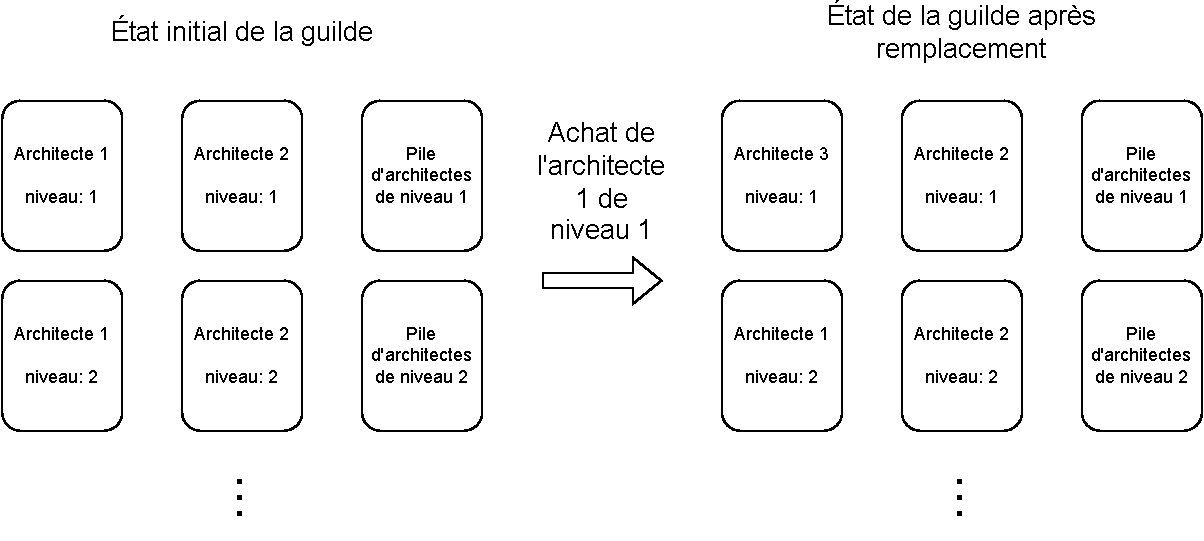
\includegraphics[width=.8\textwidth]{img/guild.pdf}
    \caption{Schéma de l'achat et remplacement d'un architecte de niveau 1}
    \label{fig:buy_builder}
\end{figure}

Les jetons sont eux stockés dans un marché et sont disposés sur un plateau carré. Pour être récupérés, les jetons doivent être pris dans le sens du chemin qui les relis.

\begin{figure}[H]
    \centering
    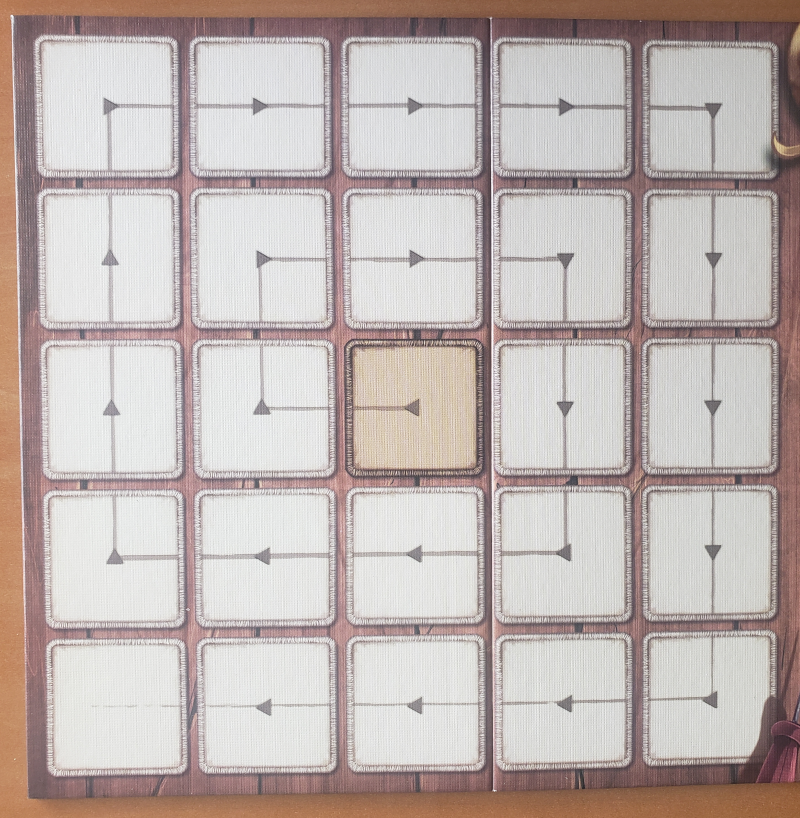
\includegraphics[width=.4\textwidth]{img/projMunificenceBoard.png}
    \caption{Image schématisant le plateau et le chemin reliant les jetons}
    \label{fig:board_example}
\end{figure}


À chaque tours, il n'est possible de faire qu'une action, on peut choisir de soit prendre entre 1 et 3 jetons dans le marché, soit d'embaucher un architecte auprès de la guilde. Lors de la prise de jetons ou de l'embauche d'un architecte, il est possible qu'un pouvoir soit attaché à ce dernier, et alors le pouvoir s'exécute à la fin de l'action.

Au début d'un tour, il est aussi possible, si on a accumulé une faveur, de l'utiliser pour prendre un jeton dans le marché ou pour renouveler les architectes disponibles d'un niveau donné de la guilde.


